\documentclass[a4paper,11pt]{report}
\usepackage{booktabs}
\renewcommand{\arraystretch}{1.3}
%-------------------------------------------------------------------------------
%	FONT
%-------------------------------------------------------------------------------
\usepackage[utf8]{inputenc}
\usepackage[T1]{fontenc}

%\usepackage[scaled=0.8]{beramono} % beramono or luximono give very nice ttfamily fonts

%-------------------------------------------------------------------------------
%	PAGE LAYOUT
%-------------------------------------------------------------------------------
\usepackage[toc,page]{appendix}

\textwidth = 410pt

\usepackage{fancyhdr}
\pagestyle{fancy}
\fancyhf{}

%\renewcommand{\sectionmark}[1]{\markright{\thesection.\ #1}}

%\nouppercase{\rightmark}

\lhead{\bfseries \nouppercase{\leftmark}}
\rhead{\bfseries \nouppercase{\rightmark}}
\lfoot{}
\rfoot{\bfseries Page \thepage}

\headwidth=1.1\textwidth
\renewcommand{\headrulewidth}{1.5pt}
\renewcommand{\footrulewidth}{1.5pt}
\fancyhfoffset[L]{24pt}
\fancyhfoffset[R]{24pt}

\fancypagestyle{plain}{%
\fancyhf{} % clear all header and footer fields
\headwidth=1.1\textwidth
\renewcommand{\headrulewidth}{1.5pt}
\renewcommand{\footrulewidth}{1.5pt}
\lhead{\bfseries \nouppercase{\leftmark}}
\rhead{\bfseries \nouppercase{\rightmark}}
%\lhead{\leftmark}
%\rhead{\rightmark}
\lfoot{}
\rfoot{\bfseries Page \thepage}
%\rfoot{Page \thepage}
\headwidth=1.1\textwidth
\fancyhfoffset[L]{24pt}
\fancyhfoffset[R]{24pt}
}

\newcommand{\mysection}[2]{%
                         \sectionmark{#1}%
                         \section{#2}%
                         \sectionmark{#1}%
                       }

%%%%%%%%%
%\renewcommand{\chaptermark}[1]{\markboth{\uppercase{\thechapter.\ #1}}{}}
%\renewcommand{\sectionmark}[1]{\markright{\uppercase{\thesection.\ #1}}}
%\newcommand{\helv}{\fontfamily{phv}\fontseries{b}\fontsize{9}{11}\selectfont}
%\lhead[\helv \thepage]{\helv \rightmark}
%\rhead[\helv \leftmark]{\helv \thepage}
%\cfoot{}
%-------------------------------------------------------------------------------
%	OTHER PACKAGES and COMMANDS
%-------------------------------------------------------------------------------
\usepackage{graphicx}
\usepackage{epstopdf}


\usepackage{float}
\usepackage{tikz}
\usepackage{tikz-uml} 
\usepackage{amsmath}

\usepackage{pifont}
\usepackage{fourier}
\usepackage{dingbat}

\usepackage{hyperref}
\usepackage{breakurl}

\newcommand{\reffig}[1]{figure \ref{fig:#1}}

\newcommand{\myparagraph}[1]{\paragraph{#1}\mbox{}\\}
%-------------------------------------------------------------------------------
%	CUSTON LISTING SETTINGS
%-------------------------------------------------------------------------------
\usepackage{listings}
\usepackage{lstcustom}
\usepackage{enumerate}
\renewcommand{\lstfontfamily}{\ttfamily}
%-------------------------------------------------------------------------------
%	COLORS
%-------------------------------------------------------------------------------

\definecolor{Lightgray}{gray}{.80}
\definecolor{lightgrey}{rgb}{0.9,0.9,0.9}


%-------------------------------------------------------------------------------
%       Commands
%-------------------------------------------------------------------------------
\newcommand{\Code}[1]{\texttt{#1}}
\newcommand{\BornAgain}{\Code{BornAgain}}%
\newcommand{\IsGISAXS}{\Code{IsGISAXS}}%
\newcommand{\SecLabel}[1]{\label{sec:#1}}%
\newcommand{\SecRef}[1]{Section~\ref{sec:#1}}% 
\newcommand{\MakeRemark}[2]
{ \noindent \smallpencil \colorbox{Lightgray}{\parbox{\dimexpr\linewidth-8\fboxsep}			{\underline{#1} #2 }}
}

\newcommand{\ImportantPoint}[2]
{\noindent
  {\huge\danger}\colorbox{Lightgray}{\parbox{\dimexpr\linewidth-8\fboxsep}
 {\underline{#1} #2}}}

\newcommand{\mychapter}[2]{
    \setcounter{chapter}{#1}
    \setcounter{section}{0}
    \chapter*{#2}
    \addcontentsline{toc}{chapter}{#2}
}

%-------------------------------------------------------------------------------
%	TITLE PAGE
%-------------------------------------------------------------------------------
\title{
{\Huge\bf BornAgain}\\[10mm]
Software for simulating and fitting\\
X-ray and neutron small-angle scattering\\
at grazing incidence\\
\vspace*{10mm} User Manual \\
\large{version 0.1.1\\\today}
\vspace*{5mm}
}

\author{ 
{\LARGE C. Durniak, G. Pospelov, W. Van Herck, J. Wuttke }\\[5mm]
\large
Scientific Computing Group\\
J\"ulich Centre for Neutron Science\\
outstation at Heinz Maier-Leibnitz Zentrum Garching\\
Forschungszentrum J\"ulich GmbH
}

\date{{}}
%License: Creative Common CC-BY-SA \\
%\today
%}


%\usepackage{eso-pic}
%\newcommand\BackgroundPic{%
%\put(0,0){%
%\parbox[b][\paperheight]{\paperwidth}{%
%\vfill
%\centering
%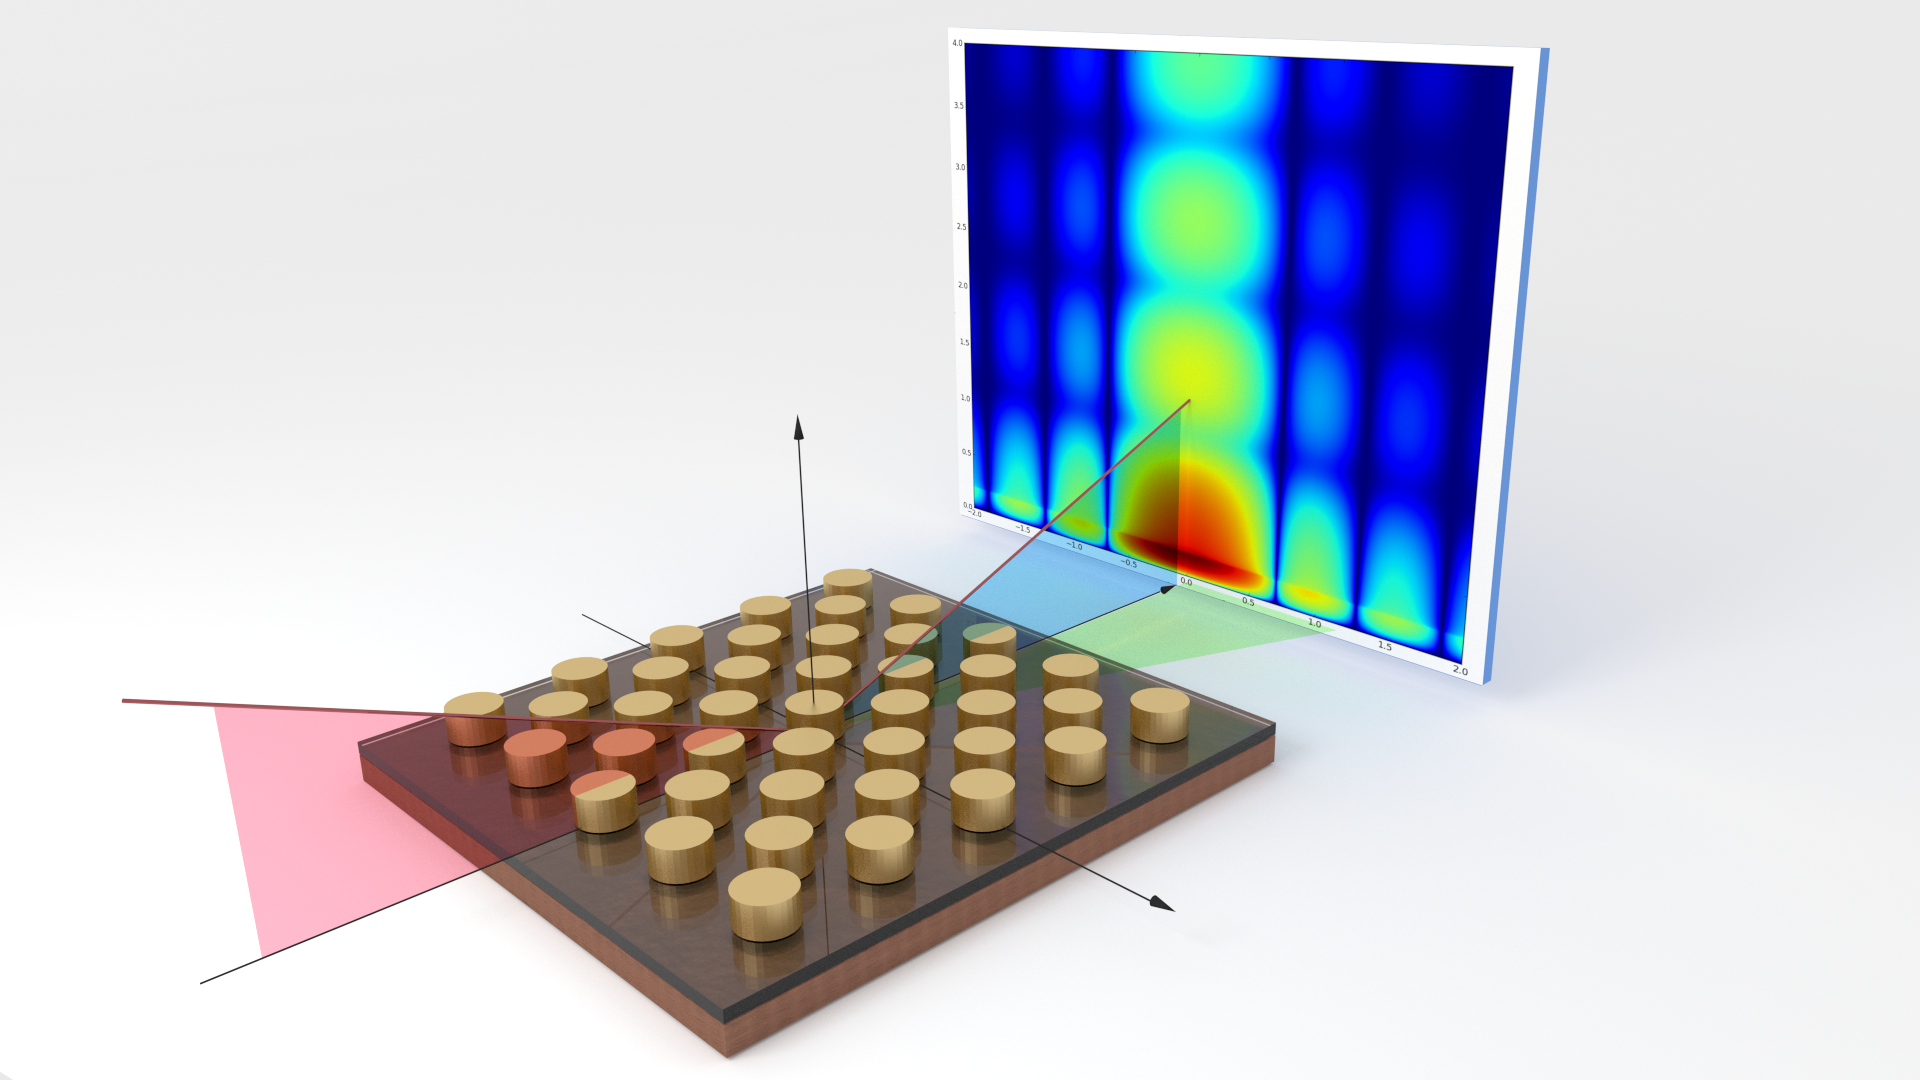
\includegraphics[width=\paperwidth,height=\paperheight,%
%keepaspectratio]{results2_2.png}%
%\vfill
%}}}


%-------------------------------------------------------------------------------
%	DOCUMENT
%-------------------------------------------------------------------------------
\begin{document}

\maketitle


\newpage

{\Huge 
\vspace*{0.5cm}
\noindent
Disclaimer
} \newline
\vspace*{0.25cm}

\noindent
{\large
This manual is under development and is not currently a comprehensive listing of
\BornAgain\ features. 
The included information and instructions are a subject to substantial change and
are provided only as a preview.
}

\tableofcontents
%\lstlistoflistings
%\listoffigures
%\listoftables
%%%%%%%%%%%%%%%%%%%%%%%%%%%%%%%%%%%%%%%%%%%%%%%%%%%%%%%%%%%%%%%%%%%%%%%%%%%%%%%%
%%
%%   BornAgain User Manual
%%
%%   homepage:   http://www.bornagainproject.org
%%
%%   copyright:  Forschungszentrum Jülich GmbH 2015
%%
%%   license:    Creative Commons CC-BY-SA
%%   
%%   authors:    Scientific Computing Group at MLZ Garching
%%               C. Durniak, M. Ganeva, G. Pospelov, W. Van Herck, J. Wuttke
%%
%%%%%%%%%%%%%%%%%%%%%%%%%%%%%%%%%%%%%%%%%%%%%%%%%%%%%%%%%%%%%%%%%%%%%%%%%%%%%%%%


\cleardoublepage
\mychapter{0}{Introduction}

\BornAgain\
%\marginpar{scope}%
is a free and open-source software package
to simulate and fit small-angle
scattering at grazing incidence (GISAS)
with X-rays (GISAXS) or neutrons (GISANS).
It provides a generic framework
for modeling multilayer samples with smooth or
rough interfaces and with various types of embedded nanoparticles.
%\marginpar{name}%
The name, \BornAgain,
alludes to the central role of the distorted-wave Born
approximation (DWBA) in the physical description of the
scattering process.
\index{Distorted-wave Born approximation}

\BornAgain\
%\marginpar{extends \IsGISAXS}
almost completely reproduces the functionality
of the widely used program \IsGISAXS\
\index{IsGISAXS@\IsGISAXS}
\index{Lazzari, R\'emi}
by R\'emi Lazzari \cite{Laz02,Laz08}.
\BornAgain\ goes beyond \IsGISAXS\ by
supporting an unrestricted number of layers and particles, 
diffuse reflection from rough layer interfaces,
particles with inner structures, neutron polarization and magnetic scattering.
Adhering to a strict object-oriented design,
\BornAgain\ provides a solid base for future extensions
in response to specific user needs.

\BornAgain\
%\marginpar{platforms}%
\index{Platform|see {Operating system}}%
\index{Operating system}%
is operating system independent.
We actively support
Linux,
\index{Linux}%
MacOS
\index{MacOS}%
and  Microsoft Windows.
\index{Windows|see {Microsoft Windows}}%
\index{Microsoft Windows}%
%\marginpar{licence}%
It is a free and open source software under
the GNU General Public License (GPL, version 3 or higher).
This documentation is released under the Creative Commons license CC-BY-SA.
When \BornAgain\ is used in preparing scientific papers,
please cite software and manual as follows:
\index{Citation}%
%\marginpar{citation}%
\begin{quote}
C.~Durniak, M.~Ganeva, G.~Pospelov, W.~Van Herck, J.~Wuttke (2015),\newline
BornAgain --- Software for simulating and fitting
X-ray and neutron small-angle scattering at grazing incidence,
version \UserManualVersionNumber,\newline
\url{http://www.bornagainproject.org}
\end{quote}

This User Manual is complementary to the online documentation
at \url{http://www.bornagainproject.org}.
It does not duplicate information that is more conveniently read online.
Therefore, Sect.~\ref{sec:online} just contains a few pointers to the web site.
The remainder of this User Manual mostly contains background
on the sample models and on the scattering theory implemented in \BornAgain,
and some documentation of the corresponding \Python\ functions.
%Sect.~\ref{sec:Simulation} describes
%the general methodology of a simulation with \BornAgain,
%and gives detailed usage examples.
%Sect.~\ref{sec:ScatteringCrosssection} explains
%which sample structures are supported in \BornAgain,
%and which physical approximations are used.
%Fitting is explained in Sect.~\ref{sec:Fitting}.
%More theoretical background is given in Appendix~\ref{app:theory}.
%Implemented particle formfactors are specified in Appendix~\ref{app:ff}.

\Warn{\indent Software and documentation are work in progress.
We cannot guarantee that they are accurate and correct.
Anyway, it is entirely in the responsibility of users
to ensure that their data interpretation is physically meaningful.
If in doubt, please contact us.}

\index{Bug reports}
We are grateful for all kind of feedback:
criticism, praise, bug reports, feature requests or contributed modules.
If questions go beyond normal user support,
we will be glad to discuss a scientific collaboration.

\newpage
\section{Quick start} \SecLabel{QuickStart}

This section shortly describes how to build \BornAgain\ from source and run first
simulation. More details about software architecture and installation
procedure are given in \SecRef{SoftwareArchitecture} and \SecRef{InstallationProcedure}. \\

\noindent
{\bf Step I: $~$ installing third party software}
\begin{itemize}
\item boost library ($\geq 1.48$)
\item GNU scientific library ($\geq 1.15$)
\item fftw3 library ($\geq 3.3.1$)
\item python-2.7, python-devel, python-numpy-devel
\item Eigen3 library ($\geq 3.1.0$), optional
\item ROOT framework ($\geq 5.34.00$), optional
\item python-matplotlib, optional
\end{itemize}
\vspace*{2mm}


\noindent
{\bf Step II: $~$ getting the source}
\begin{lstlisting}[language=bash, style=commandline]
git clone git://apps.jcns.fz-juelich.de/BornAgain.git 
\end{lstlisting}
\vspace*{3mm}


\noindent
{\bf Step III: $~$ building the source}
\begin{lstlisting}[language=shell, style=commandline]
mkdir <build_dir>; cd <build_dir>;
cmake <source_dir> -DCMAKE_INSTALL_PREFIX=<install_dir>
make
make check
make install
\end{lstlisting}
\vspace*{3mm}


\noindent
{\bf Step IV: $~$ running example}
\begin{lstlisting}[language=shell, style=commandline]
cd <install_dir>/Examples/python/ex001_CylindersAndPrisms
python CylindersAndPrisms.py
\end{lstlisting}


%Requirements

%Hardware
%BornAgain is known to work on following platforms:
%Linux (x86, amd64)
%MacOS X (x86)

%Software
%GCC 4.1.2 or above   C/C++ compiler
%or
%clang
%gcc 4.1.2 or above, clang

\newpage
\section{Installation} \SecLabel{Installation}

This section describes how to build and install \BornAgain\ libraries from the source.
At the moment we support building on x86/x86\_64 Linux and Mac OS X operating systems.
Support for Windows systems is planned in next releases.
%In the later releases we are planing to include support for Windows systems and provide
%binary distributions for major Windows/Mac/Linux.
There are three major steps to building \BornAgain\ :
\begin{enumerate}[1.]
\item Acquire required third-party libraries.
\item Get \BornAgain\ source code.
\item Use \Code{cmake} to build and install software.
\end{enumerate}
The remainder of this section explains each step in detail.

\subsection{Third-party software.}
To successfully build \BornAgain\ a number of prerequisite packages must be installed.

\begin{itemize}
\item compilers: clang  versions $\geq 3.1$ or GCC versions $\geq 4.2$
\item cmake ($\geq 2.8$)
\item boost library ($\geq 1.48$)
\item GNU scientific library ($\geq 1.15$)
\item fftw3 library ($\geq 3.3$)
\item python ($\geq 2.7$), python-devel, python-numpy-devel
\end{itemize}
\vspace*{2mm}

Other packages are optional
\begin{itemize}
\item ROOT framework (adds several additional fitting algorithms to \BornAgain)
\item python-matplotlib (allows to run usage examples with graphics)
%\item Eigen3 library ($\geq 3.1.0$)
\end{itemize}

All required packages can be easily installed on most Linux distributions using the system's package
manager. Below we give a few examples for several selected operation systems. Please note,
that other distributions (Fedora, Mint, etc) may have different commands for invoking the package manager and slightly different names of packages (like ``boost'' instead of ``libboost'' etc). Besides that, the installation should be very similar.
\vspace*{3mm}

% ---------------
%  OpenSuse 12.3
% ---------------
\noindent
{\large\bf OpenSuse 12.3} \newline
Adding ``scientific'' repository 
\begin{lstlisting}[language=shell, style=commandline]
sudo zypper ar http://download.opensuse.org/repositories/science/openSUSE_12.3 science
\end{lstlisting}

\noindent
Installing required packages
\begin{lstlisting}[language=shell, style=commandline]
sudo zypper install git-core cmake gsl-devel boost-devel fftw3-devel python-devel python-numpy-devel
\end{lstlisting}

\noindent
Installing optional packages
\begin{lstlisting}[language=shell, style=commandline]
sudo zypper install libroot-* root-plugin-* root-system-* root-ttf libeigen3-devel python-matplotlib
\end{lstlisting}
\vspace*{3mm}


% ---------------
%  Ubuntu 13.04
% ---------------
\noindent
{\large\bf Ubuntu 13.04} \newline
Installing required packages
\begin{lstlisting}[language=shell, style=commandline]
sudo apt-get install git cmake libgsl0-dev libboost-all-dev libfftw3-dev python-dev python-numpy
\end{lstlisting}

\noindent
Installing optional packages
\begin{lstlisting}[language=shell, style=commandline]
sudo apt-get install libroot-* root-plugin-* root-system-* ttf-root-installer libeigen3-dev python-matplotlib python-matplotlib-tk
\end{lstlisting}
\vspace*{3mm}


% ---------------
%  MacOS 10.8
% ---------------
\noindent
\noindent
{\large\bf Mac OS X 10.8} \newline
To simplify the installation of third party open-source software on a Mac OS X system we recommend the use of \Code{MacPorts} package manager. 
The easiest way to install MacPorts is by downloading the \Code{dmg} 
from \url{www.macports.org/install.php} and running the system's installer.
After the installation new command ``\Code{port}'' will be available in terminal window of your Mac. \

\noindent
Installing required packages
\begin{lstlisting}[language=shell, style=commandline]
sudo port -v selfupdate
sudo port install git-core cmake
sudo port install fftw-3 gsl
sudo port install boost -no_single-no_static+python27 


\end{lstlisting}

\noindent
Installing optional packages
\begin{lstlisting}[language=shell, style=commandline]
sudo port install py27-matplotlib py27-numpy py27-scipy
sudo port install root +fftw3+python27
sudo port install eigen3
\end{lstlisting}




\subsection{Getting source code}
\BornAgain\ source can be downloaded at \url{http://apps.jcns.fz-juelich.de/BornAgain}
and unpacked with
\begin{lstlisting}[language=shell, style=commandline]
tar xfz bornagain-<version>.tgz
\end{lstlisting}

\noindent
Alternatively one can obtain \BornAgain\ source from our public Git repository.
\begin{lstlisting}[language=bash, style=commandline]
git clone git://apps.jcns.fz-juelich.de/BornAgain.git 
\end{lstlisting}
\vspace*{3mm}


\noindent
{\bf\large More about Git} \\
Our Git repository holds two main branches called ``master'' and ``develop''. We consider ``master''
branch to be the main branch where the source code of HEAD always reflects latest stable release. \Code{git clone} command shown above
\begin{enumerate}[1.]
\item gives you a source code snapshot corresponding to the latest stable release,
\item automatically sets up your local master branch to track our remote master branch, 
so you will be able to fetch changes from the remote branch at any time using ``git pull'' command.
\end{enumerate}

Master branch is updating approximately once per month.
% that reflects our release cycle.
The second branch, ``develop'' branch, is a snapshot of the current development.
This is where any automatic nightly builds are built from. The develop branch is
always expected to work, so to get the most recent features one can switch source code to it by
\begin{lstlisting}[language=bash, style=commandline]
cd BornAgain
git checkout develop
git pull
\end{lstlisting}
\vspace*{3mm}



\subsection{Building and installing the code}

\BornAgain\ should be build using \Code{CMake} cross platform build system. 
Having third-party libraries installed on the system and \BornAgain\ source code acquired as was explained in
previous sections, type build commands
\begin{lstlisting}[language=bash, style=commandline]
mkdir <build_dir>
cd <build_dir>
cmake <source_dir> -DCMAKE_INSTALL_PREFIX=<install_dir>
make
\end{lstlisting}
\vspace*{3mm}

Here \Code{<source\_dir>} is the name of directory, where \BornAgain\ source code has been
copied, \Code{<install\_dir>} is the directory, where user wants  the package
to be installed, and \Code{<build\_dir>} is the directory where building will occur.

\MakeRemark{About \Code{CMake}}{
\\Having dedicated directory \Code{<build\_dir>} for build process
is recommended by \Code{CMake}. That allows several builds with different compilers/options from the same source and keeps source directory clean from build remnants. \\
}


Compilation process invoked by the command ``make'' lasts about 10 min for an average laptop
of 2012 edition. On multi-core machines the compilation time  can be decreased by invoking command
``make'' with the parameter ``make -j[N]'', where N is the number of cores.

Running functional tests is an optional but recommended step. Command ``make check''
will compile several additional tests and run them one by one. Every test contains
the simulation of a typical GISAS geometry and the comparison on numerical level of simulation results with reference files. Having 100\% tests passed ensures that your local installation
is correct.
\begin{lstlisting}[language=bash, style=commandline]
make check
...
100% tests passed, 0 tests failed out of 26
Total Test time (real) = 89.19 sec
[100%] Build target check
\end{lstlisting}
\vspace*{3mm}


The last command ``make install'' copies compiled libraries and some usage examples
into  the installation directory.
\begin{lstlisting}[language=bash, style=commandline]
make install
\end{lstlisting}


\subsubsection{Troubleshooting}

In the case of complex system setup, with variety of libraries of different versions 
scattered across multiple places (\Code{/opt/local}, \Code{/usr} etc.),
you may want to help \Code{CMake} to find libraries in proper place. 
In example below
two system variables are defined to force \Code{CMake} to prefer libraries
found in \Code{/opt/local} to other places.
\begin{lstlisting}[language=bash, style=commandline]
export CMAKE_LIBRARY_PATH=/opt/local/lib:$CMAKE_LIBRARY_PATH
export CMAKE_INCLUDE_PATH=/opt/local/include:$CMAKE_INCLUDE_PATH
\end{lstlisting}


If compilation fails for some reason, please submit your bug report including compilation errors
at \url{http://apps.jcns.fz-juelich.de/redmine/projects/bornagain/issues}



\subsection{What is next?}

In your installation directory you will find
\begin{lstlisting}[language=bash, style=commandline]
./include - header files for compilation of your C++ program
./lib - libraries to import into python or link with your C++ program
./Examples - directory with examples
\end{lstlisting}

Run your first example and enjoy first BornAgain simulation plot.
\begin{lstlisting}[language=bash, style=commandline]
cd <install_dir>/Examples/python/ex001_CylindersAndPrisms
python CylindersAndPrisms.py
\end{lstlisting}








%%%%%%%%%%%%%%%%%%%%%%%%%%%%%%%%%%%%%%%%%%%%%%%%%%%%%%%%%%%%%%%%%%%%%%%%%%%%%%%%
%%
%%   BornAgain User Manual
%%
%%   homepage:   http://www.bornagainproject.org
%%
%%   copyright:  Forschungszentrum Jülich GmbH 2015
%%
%%   license:    Creative Commons CC-BY-SA
%%   
%%   authors:    Scientific Computing Group at MLZ Garching
%%               C. Durniak, M. Ganeva, G. Pospelov, W. Van Herck, J. Wuttke
%%
%%%%%%%%%%%%%%%%%%%%%%%%%%%%%%%%%%%%%%%%%%%%%%%%%%%%%%%%%%%%%%%%%%%%%%%%%%%%%%%%


\mysection{Example 1: two types of islands on a substrate without interference}{Example 1: two types of islands on top of
  substrate without interference} \SecLabel{Example1Python}

%\section{Example 1: two types of islands on top of
%  substrate without interference.} \SecLabel{Example1Python}

% \sectionmark{Example 1}

In this example, we simulate the scattering from a mixture of
cylindrical and prismatic nanoparticles without any interference
between them. These particles are placed in air, on top
of a substrate.\\ We are going to go through each step of the
simulation. The \Python\ code snippet specific to each stage will be given at
the beginning of the description. 
More examples can be found at our project web site \url{http://www.bornagainproject.org/documentation/python_examples}

% But for the sake of completeness the full code is given
% in Appendix~\ref{PythonSimulationExampleScript}.


% -----------------------------------------------------------------------------
%
% -----------------------------------------------------------------------------
\subsubsection{Importing Python modules}
\begin{lstlisting}[language=python, style=eclipseboxed,name=ex1,nolol]
import numpy @\label{import_lib_beg}@
import matplotlib
import pylab @\label{import_lib_end}@
from bornagain import * @\label{import_ba}@
\end{lstlisting}
We start by importing different functions from external
modules, for example \Code{NumPy} (lines~\ref{import_lib_beg}-\ref{import_lib_end}), which
is a fundamental package for scientific computing with \Python\
\cite{s:numpy}.  In particular, line~\ref{import_ba}
imports the features of \BornAgain\ software.


% -----------------------------------------------------------------------------
%
% -----------------------------------------------------------------------------
\subsubsection{Defining the materials} 
\begin{lstlisting}[language=python, style=eclipseboxed,name=ex1,nolol]
def get_sample(): @\label{def_function}@
    """
    Build and return the sample representing cylinders and pyramids on top of substrate without interference.
   """
    # defining materials @\label{material1}@
    m_air = HomogeneousMaterial("Air", 0.0, 0.0)  @\label{material2}@
    m_substrate = HomogeneousMaterial("Substrate", 6e-6, 2e-8) @\label{material3}@
    m_particle = HomogeneousMaterial("Particle", 6e-4, 2e-8) @\label{materialparticle}@

\end{lstlisting}
Line~\ref{def_function} marks the beginning of the
function to define our sample. Lines~\ref{material2}, \ref{material3} and \ref{materialparticle} define different
materials using class \Code{HomogeneousMaterial}. The general syntax is the following 
\begin{lstlisting}[language=python, style=eclipse,numbers=none]
<material_name> = HomogeneousMaterial("name", delta, beta)
\end{lstlisting}
where \Code{name} is the name of the
material associated with its complex refractive index
n=1-\Code{delta} +i \Code{beta}. \Code{<material\_name>} is later used when
referring to this particular material. The three materials defined in this example are \Code{Air} with a refractive
index of 1 (\Code{delta = beta = 0}), a \Code{Substrate} associated with a complex refractive index
equal to $1-6\times 10^{-6} +i2\times 10^{-8} $, and the material of the particles, whose refractive index is \Code{n}$=1-6\times 10^{-4}+i2\times 10^{-8}$.


% -----------------------------------------------------------------------------
%
% -----------------------------------------------------------------------------
\subsubsection{Defining the particles}
\begin{lstlisting}[language=python,style=eclipseboxed,name=ex1,nolol]
    # collection of particles @\label{particles1}@
    cylinder_ff = FormFactorCylinder(5*nanometer, 5*nanometer) @\label{particlescyl1}@
    cylinder = Particle(m_particle, cylinder_ff) @\label{particlescyl2}@
    prism_ff = FormFactorPrism3(10*nanometer, 5*nanometer) @\label{particlesprism1}@
    prism = Particle(m_particle, prism_ff) @\label{particlesprism2}@
\end{lstlisting}
We implement two different shapes of particles: cylinders and
prisms (\textit{i.e.} elongated particles with a constant equilateral triangular cross section).
 
All particles implemented in \BornAgain\ are defined by their
form factors (see Appendix~\ref{app:ff}), their sizes and the material
they are made of. Here, for the
cylindrical particle, we input its radius and height.  For the prism, 
the possible inputs are the length of one side of its equilateral triangular
base and its height.

In order to define a particle, we proceed in two steps. For example for
the cylindrical particle, we first specify the form factor of a cylinder with 
its radius and height, both equal to 5 nanometers in this particular
case (see line~\ref{particlescyl1}). Then we associate this shape with
the constituting material as in line~\ref{particlescyl2}.
The same procedure has been applied for the prism in lines~\ref{particlesprism1} and \ref{particlesprism2}, respectively.


% -----------------------------------------------------------------------------
%
% -----------------------------------------------------------------------------
\subsubsection{Characterizing particles assembly} 
\begin{lstlisting}[language=python, style=eclipseboxed, name=ex1,nolol]
    particle_layout = ParticleLayout()  @\label{particlesdecor1}@
    particle_layout.addParticle(cylinder, 0.0, 0.5)  @\label{particlesdecor2}@
    particle_layout.addParticle(prism, 0.0, 0.5)@\label{particlesdecor3}@
    interference = InterferenceFunctionNone()  @\label{particlesnointerf}@
    particle_layout.addInterferenceFunction(interference)  @\label{particlesinterf}@
\end{lstlisting}
The object which holds the information about the positions and densities of particles
in our sample is called \Code{ParticleLayout}
(line~\ref{particlesdecor1}). We use the associated function \Code{addParticle}
for each particle shape (lines~\ref{particlesdecor2}, \ref{particlesdecor3}). Its general syntax is 

\begin{lstlisting}[language=python, style=eclipse,numbers=none]
addParticle(<particle_name>, depth, abundance) 
\end{lstlisting}
where \Code{<particle\_name>} is the name used to define the particles
(lines~\ref{particlescyl2} and \ref{particlesprism2}), \Code{depth}
(default value = 0)
is the vertical position, expressed in nanometers, of the particles in a given layer (the
association with a particular layer will be done during the next step) and
\Code{abundance} is the proportion of this type of particles, 
normalized to the total number of particles. Here we have 50\% of cylinders
and 50\% of prisms.

\ImportantPoint{Remark:}{Depth of particles\\
The vertical positions of the particles in a layer are given in relative
coordinates. For the top layer, the bottom of the layer corresponds to
\Code{depth}=0 and negative values would correspond to particles
floating above layer 1 since the vertical axis, shown in \reffig{multil3d} is pointing upwards. But for all the other layers, it is the top of the
layer which corresponds to \Code{depth}=0.}\\


\noindent Finally, lines~\ref{particlesnointerf} and
\ref{particlesinterf} specify that there is \textbf{no coherent interference} between
the waves scattered by these particles. In this case, the intensity is calculated by
the incoherent sum of the scattered waves: $\langle |F_j|^2\rangle$,
where $F_j$ is the form factor associated with the particle of type $j$.  The way these waves
interfere imposes the horizontal distribution of
the particles as
the interference reflects the long or short-range order of the
particles distribution (see  \SecRef{sect:interf}). On the contrary, the vertical position is
imposed when we add the particles in a given layer by parameter \Code{depth}, as shown in lines~\ref{particlesdecor2} and \ref{particlesdecor3}.


% -----------------------------------------------------------------------------
%
% -----------------------------------------------------------------------------
\subsubsection{Multilayer}
\begin{lstlisting}[language=python, style=eclipseboxed,name=ex1,nolol]
# air layer with particles and substrate form multi layer  @\label{sampleassembling}@
    air_layer = Layer(m_air) @\label{airlayer}@
    air_layer.addLayout(particle_layout) @\label{airlayerdecorator}@
    substrate_layer = Layer(m_substrate, 0)  @\label{substratelayer}@
    multi_layer = MultiLayer() @\label{multilayercanvas}@
    multi_layer.addLayer(air_layer) @\label{layerairdecor}@
    multi_layer.addLayer(substrate_layer) @\label{layersubstrate}@
    return multi_layer @\label{returnmlayer}@
\end{lstlisting}
We now have to configure our sample. For this first example,
the particles, \textit{i.e.} cylinders and prisms, are on top of a substrate in an
air layer. \textbf{The order in which we define these layers is important: we
start from the top layer down to the bottom one}.

Let us start with the air layer. It contains the particles. In
line~\ref{airlayer}, we use the previously defined \Code{mAmbience}
(="air" material) (line~\ref{material2}). The command in line~\ref{airlayerdecorator} shows that this layer contains particles
which are defined using particle layout object. The substrate layer
only contains the substrate material (line~\ref{substratelayer}).
%Note that the
%\Code{depth} is referenced to the bottom of the top layer (negative
%values would correspond to particles floating above layer 1 as
%the vertical axis is pointing upwards). 
 
There are different possible syntaxes to define a layer. As shown in
lines~\ref{airlayer} and \ref{substratelayer}, we can use
\Code{Layer(<material\_name>,thickness)} or
\Code{Layer(<material\_name>)}. The second case corresponds
to the default value of the \Code{thickness}, equal to 0. The \Code{thickness} is
expressed in  nanometers.

Our two layers are now fully characterized. The sample is assembled using
\Code{MultiLayer()} constructor (line~\ref{multilayercanvas}): we start with the air layer decorated
with the particles (line~\ref{layerairdecor}), which is the layer at
the top and end with the bottom layer, which is the
substrate (line~\ref{layersubstrate}).


% -----------------------------------------------------------------------------
%
% -----------------------------------------------------------------------------
\subsubsection{Characterizing the input beam and
output detector}

\begin{lstlisting}[language=python, style=eclipseboxed,name=ex1,nolol]
def get_simulation():  @\label{run1}@
    """
    Create and return GISAXS simulation with beam and detector defined
    """
    simulation = Simulation() @\label{run2}@
    simulation.setDetectorParameters(100, -1.0*degree, 1.0*degree, 100, 0.0*degree, 2.0*degree) @\label{rundetector}@
    simulation.setBeamParameters(1.0*angstrom, 0.2*degree, 0.0*degree) @\label{runbeam}@
    return simulation @\label{returnsimul}@
\end{lstlisting}
The first stage is to create the \Code{Simulation()} object (line~\ref{run2}). Then we define the detector (line~\ref{rundetector}) and beam
parameters (line~\ref{runbeam}). %, which are associated with the
%sample previously defined (line~\ref{runsample}). Finally we run
%the simulation (line~\ref{runsimul}). 
Those functions are part of the Simulation
class.  The different incident and exit angles are
shown in \reffig{multil3d}.

The detector parameters are set using ranges of angles via
the function:

\begin{lstlisting}[language=python, style=eclipse,numbers=none]
setDetectorParameters(n_phi, phi_f_min, phi_f_max, n_alpha, alpha_f_min, alpha_f_max),
\end{lstlisting}


\noindent where number of bins \Code{n\_phi}, low edge of first bin \Code{phi\_f\_min} and
upper edge of last bin \Code{phi\_f\_max} all together define $\phi_f$ detector axis, 
while \Code{n\_alpha}, \Code{alpha\_f\_min} and \Code{alpha\_f\_max} are related to 
$\alpha_f$ detector axis.

\ImportantPoint{Remark:}{Axis binning\\
By default axes are binned to provide constant bin size in k-space, which means slightly
non-equidistant binning in angle space. Other possible options, including user defined
axes with custom variable bin size are explained elsewhere.
}
\vspace*{2mm}


%are the minimum and maximum values of $\phi_f$, respectively, \Code{n\_alpha} is
%the number of bins for $\alpha_f$ axis, \Code{alpha\_f\_min} and \Code{alpha\_f\_max} 
%are the minimum and maximum values of
%$\alpha_f$, respectively.

%\Code{isgisaxs\_style=True} (default value = \Code{False}) is a boolean
%used to characterise the structure of the output data. If
%\Code{isgisaxs\_style=True}, the output data is binned at constant
%values of the sine of the output angles, $\alpha_f$ and $\phi_f$, otherwise it is binned
%at constant values of these two angles.\\



\noindent To characterize the beam we use function 
\begin{lstlisting}[language=python, style=eclipse,numbers=none]
setBeamParameters(lambda, alpha_i, phi_i),
\end{lstlisting}

\noindent where \Code{lambda} is the incident beam wavelength,
\Code{alpha\_i} is the incident
grazing angle on the surface of the sample,
\Code{phi\_i} is the in-plane
direction of the incident beam (measured with respect to the $x$-axis).

\ImportantPoint{Remark:}{Scattering vector\\
In \BornAgain\, the wave vector $\mathbf{q}$ is defined as
$\mathbf{k}_i -\mathbf{k}_f$, where $\mathbf{k}_i$ is the incident
wave vector and $\mathbf{k}_f$ the scattered one.}

%\noindent \underline{Remark}: Note that, except for
%\Code{isgisaxs\_style}, there are no default values implemented for the
%parameters of the beam and detector.\\

%\noindent Line~\ref{runsimul} shows the command to run the simulation using the
%previously defined setup.
%%%%%%%%%%%%%


% -----------------------------------------------------------------------------
%
% -----------------------------------------------------------------------------
\subsubsection{Running the simulation  and
  plotting the results}

\begin{lstlisting}[language=python, style=eclipseboxed,name=ex1,nolol]
def run_simulation(): @\label{run_simulation}@
    """
   Run simulation and plot results
    """
    sample = get_sample() @\label{get_sample}@
    simulation = get_simulation() @\label{get_simulation}@
    simulation.setSample(sample)  @\label{setsample}@
    simulation.runSimulation()  @\label{runsimul}@
    result = simulation.getIntensityData().getArray() + 1  # for log scale  @\label{outputdata}@
    pylab.imshow(numpy.rot90(result, 1), norm=matplotlib.colors.LogNorm(), extent=[-1.0, 1.0, 0, 2.0]) @\label{plot1}@
    pylab.show() @\label{plot2}@
\end{lstlisting}
%In function \Code{run\_simulation()}, we associate the sample
%characterised by function \Code{get\_sample()} with the input beam and
%output detector, defined in function \Code{get\_simulation()} (line~\ref{runsample}).
The function, whose definition starts from line~\ref{run_simulation}, gathers all
items. We create the sample and the simulation objects at the lines 
~\ref{get_sample} and \ref{get_simulation}, using calls to the previously defined functions. We assign the sample to the simulation at line ~\ref{setsample} and
finally launch the simulation at line ~\ref{runsimul}.

In line~\ref{outputdata} we obtain the simulated intensity
as a function of outgoing angles $\alpha_f$ and $\phi_f$ for further
uses (plots, fits,\ldots) as a \Code{NumPy} array containing
\Code{n\_phi}$\times$\Code{n\_alpha}
datapoints. Lines~\ref{plot1}-\ref{plot2} produces the two-dimensional
contour plot of the intensity as a function of $\alpha_f$ and
$\phi_f$ shown in \reffig{output_ex1}. 

\begin{figure}[htbp]
  \begin{center}
   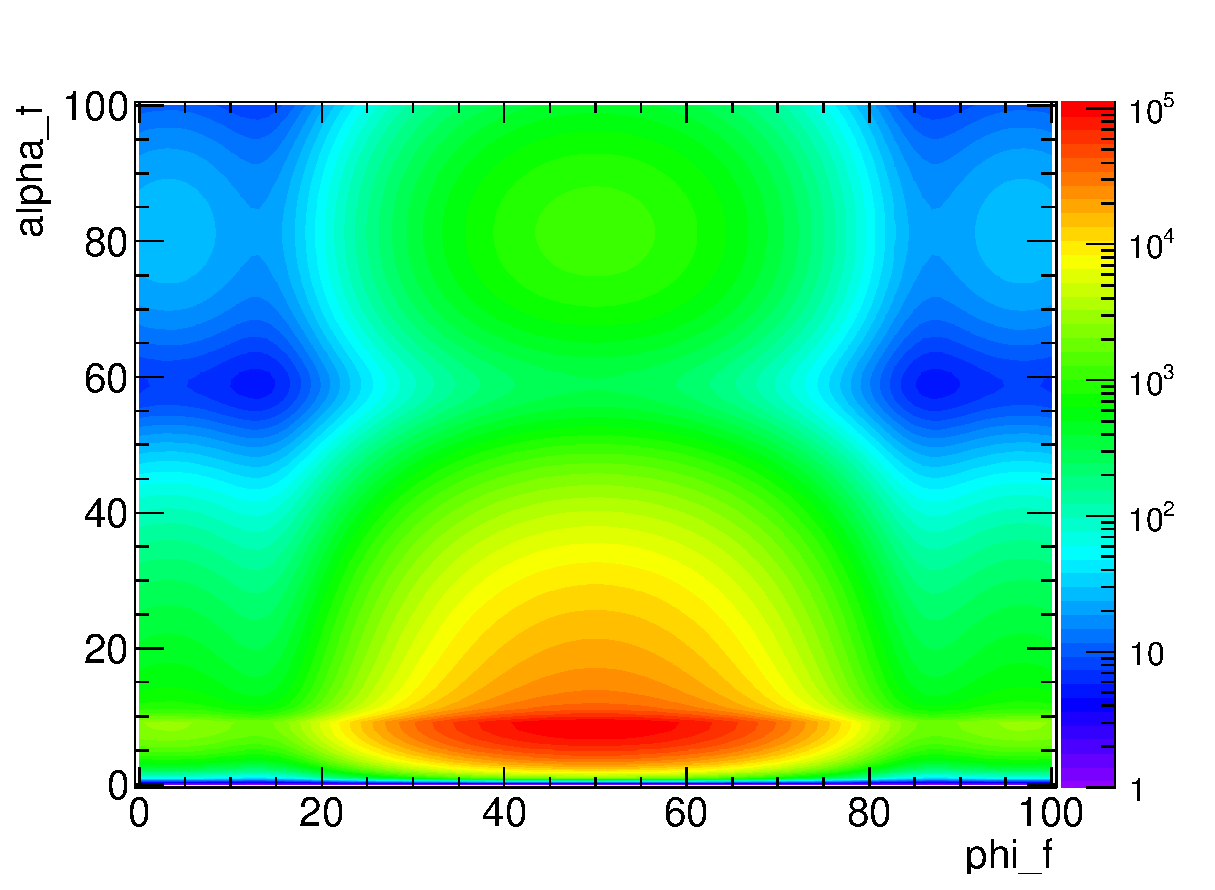
\includegraphics[clip=true, width=120mm]{Figures/gisasmap/Manual_ex1.eps}
  \end{center}
  \caption[Example 1: Simulated grazing-incidence small-angle X-ray scattering from a mixture of
cylindrical and prismatic nanoparticles without any interference, deposited on top
of a substrate]{Simulated grazing-incidence small-angle X-ray scattering from a mixture of
cylindrical and prismatic nanoparticles without any interference, deposited on top
of a substrate. The input beam is characterized by a wavelength
$\lambda$ of 1~\AA\ and incident angles $\alpha_i=0.2^{\circ}$, $\phi_i=0^{\circ}$. The
cylinders have a radius and a height both equal to 5~nm, the prisms
are characterized by a side length equal to 10~nm and they are 5~nm high. The
material of the particles has a refractive index of $1-6\times 10^{-4}+i2\times 10^{-8}$. For the substrate
it is equal to $1-6\times 10^{-6} +i2\times 10^{-8} $. The color scale
is associated with the output intensity in arbitrary units. }
\label{fig:output_ex1}
\end{figure}



%%%%%%%%%%%%%%%%%%%%%%%%%%%%%%%%%%%%%%%%%%%%%%%%%%%%%%%%%%%%%%%%%%%%%%%%%%%%%%%
%
%%%%%%%%%%%%%%%%%%%%%%%%%%%%%%%%%%%%%%%%%%%%%%%%%%%%%%%%%%%%%%%%%%%%%%%%%%%%%%%
\section{Example 2: working with sample parameters} \SecLabel{WorkingWithSampleParameters}

This section gives additional details about the manipulation of sample parameters
during run time; that is after the sample has already been constructed. 
For a single simulation this is normally not necessary. However it might be useful
during interactive work when the user tries to find optimal sample parameters by
running a series of simulations.
A similar task also arises when the theoretical model, composed of the
description of the sample and of the simulation, is used for fitting real data.
In this case, the fitting kernel requires a list of the existing sample parameters
and a mechanism for changing the values of these parameters in order to find 
their optima.

In \BornAgain\ this is done using the so-called sample parameter pool
mechanism. We are going to briefly explain this approach using the example
of \SecRef{Example1Python}.

In \BornAgain\ a sample is described by a hierarchical tree of objects.
For the multilayer created in the previous section this tree can be graphically
represented as shown in Fig.~\ref{fig:sample_tree}. Similar trees can
be printed in a \Python\
session by running \Code{multi\_layer.printSampleTree()}

\begin{figure}[p!]

\tikzstyle{every node}=[draw=black,thick,anchor=west]
\tikzstyle{selected}=[draw=red,fill=red!30]
\tikzstyle{optional}=[dashed,fill=gray!50]
\begin{tikzpicture}[%
  grow via three points={one child at (0.5,-0.7) and
  two children at (0.5,-0.7) and (0.5,-1.4)},
  edge from parent path={(\tikzparentnode.south) |- (\tikzchildnode.west)}]
  \node {MultiLayer}
    child { node {Layer \#0}
		child { node {ParticleLayout } 
			child { node {Particle Info 0} 
				child {node {Particle }  
					child { node {FormFactorCylinder} 
						child { node [optional] { radius:5.0} }					
						child { node [optional] { height:5.0} }					
					}				
				}
    			child [missing] {}		
    			child [missing] {}		
			    child [missing] {}		
				child {node [optional] { abundance:0.5} }			
				child {node [optional] { depth:0.0} }			
			}
    		child [missing] {}		
    		child [missing] {}		
			child [missing] {}		
    		child [missing] {}		
    		child [missing] {}		
			child [missing] {}		
			child { node {Particle Info 1} 
				child {node {Particle }  
					child { node {FormFactorPrism3} 
						child { node [optional] { length:10.0} }					
						child { node [optional] { height:5.0} }					
					}				
				}
    			child [missing] {}		
    			child [missing] {}		
			    child [missing] {}		
				child {node [optional] { abundance:0.5} }			
				child {node [optional] { depth:0.0} }						
			}					
		}
		child [missing] {}		
   		child [missing] {}		
	    child [missing] {}		
		child [missing] {}		
   		child [missing] {}		
	    child [missing] {}		
	    child [missing] {}		
		child [missing] {}		
   		child [missing] {}		
	    child [missing] {}		
		child [missing] {}		
   		child [missing] {}		
	    child [missing] {}		
	    child [missing] {}		
		child {node [optional] { thickness:0.0} }				
    }
	child [missing] {}		
   	child [missing] {}		
	child [missing] {}		
   	child [missing] {}		
	child [missing] {}		
	child [missing] {}		
   	child [missing] {}		
	child [missing] {}		
   	child [missing] {}		
	child [missing] {}		
	child [missing] {}		
   	child [missing] {}		
	child [missing] {}		
   	child [missing] {}		
	child [missing] {}		
	child [missing] {}		
	child { node {Layer interface \#0} 
    	child {node { roughness} 
    		child {node [optional] { corrlength:0.0} }				    	
    		child {node [optional] { hurst:0.0} }				    	
    		child {node [optional] { sigma:0.0} }				    	
    	}					
	}
   	child [missing] {}		
	child [missing] {}		
	child [missing] {}		
    child { node {Layer \#1}
    	child {node [optional] { thickness:0.0} }				
    }
	child [missing] {}		
    child { node [optional] {CrossCorrLength:0.0} };
    
\end{tikzpicture}
\caption{Tree representation of the sample structure.}
\label{fig:sample_tree}
\end{figure}


The top \Code{MultiLayer} object is composed of three children, namely
\Code{Layer \#0, Layer Interface \#0} and \Code{Layer \#1}. The
children objects might themselves also be decomposed into tree-like structures. For example,
\Code{Layer \#0} contains a \Code{ParticleLayout} object, which holds information
related to the two types of particles populating the layer. All numerical values used
during the sample construction (thickness of layers, size of particles, roughness parameters) are part of the same tree structure. 
They are marked in the figure with shaded gray boxes.

These values are registered in the sample parameter pool using the name
composed of the corresponding nodes' names. And they can be accessed/changed
during run time. For example, the \Code{height} of the cylinders
populating the first layer can be changed from the
current value of $5~\rm{nm}$ to $1~\rm{nm}$ by running the command

\begin{lstlisting}[language=shell, style=commandline]
multi_layer.setParameterValue('/MultiLayer/Layer0/ParticleLayout/ParticleInfo0/Particle/FormFactorCylinder/height', 1.0)
\end{lstlisting}


A list of the names and values of all registered sample's parameters
can be displayed using the command 

\begin{lstlisting}[language=shell, style=commandline]
> multi_layer.printParameters()
The sample contains following parameters ('name':value)
'/MultiLayer/Layer0/ParticleLayout/ParticleInfo0/Particle/FormFactorCylinder/height':5
'/MultiLayer/Layer0/ParticleLayout/ParticleInfo0/Particle/FormFactorCylinder/radius':5
'/MultiLayer/Layer0/ParticleLayout/ParticleInfo0/abundance':0.5
'/MultiLayer/Layer0/ParticleLayout/ParticleInfo0/depth':0
'/MultiLayer/Layer0/ParticleLayout/ParticleInfo1/Particle/FormFactorPrism3/length':5
'/MultiLayer/Layer0/ParticleLayout/ParticleInfo1/Particle/FormFactorPrism3/height':5
'/MultiLayer/Layer0/ParticleLayout/ParticleInfo1/abundance':0.5
'/MultiLayer/Layer0/ParticleLayout/ParticleInfo1/depth':0
'/MultiLayer/Layer0/thickness':0
'/MultiLayer/Layer1/thickness':0
'/MultiLayer/LayerInterface/roughness/corrlength':0
'/MultiLayer/LayerInterface/roughness/hurst':0
'/MultiLayer/LayerInterface/roughness/sigma':0
'/MultiLayer/crossCorrLength':0
\end{lstlisting}

Wildcards \Code{'*'} can be used to reduce typing or to work on a group
of parameters. In the example below, the first command will change the
height of all cylinders in the same way, as in the previous example. The second line will change simultaneously the height of {\it both} cylinders and prisms.
\begin{lstlisting}[language=shell, style=commandline]
multi_layer.setParameterValue('*FormFactorCylinder/height', 1.0)
multi_layer.setParameterValue('*height', 1.0)
\end{lstlisting}

The complete example described in this section can be found at 
\begin{lstlisting}[language=shell, style=commandline]
./Examples/python/fitting/ex001_SampleParametersIntro/SampleParametersIntro.py
\end{lstlisting}






\section{Basic Python fitting example} \SecLabel{FittingExamples}

In this section we are going to go through a complete example of
fitting using \BornAgain. Each  step will be associated with a
detailed piece of code written in \Python. 
The complete listing of
the script is given in Appendix (see Listing~\ref{PythonFittingExampleScript}).
The script can also be found at
\begin{lstlisting}[language=shell, style=commandline]
./Examples/python/fitting/ex002_FitCylindersAndPrisms/FitCylindersAndPrisms.py
\end{lstlisting}

\noindent
This example uses the same sample geometry as in \SecRef{Example1Python}.
Cylindrical and
prismatic particles in equal proportion are deposited on a substrate layer, with no interference
between the particles. We consider the following parameters to be unkown
\begin{itemize}
\item the radius of cylinders,
\item the height of cylinders,
\item the length of the prisms' triangular basis,
\item the height of prisms.
\end{itemize}

Our reference data are a ``noisy'' two-dimensional intensity
map obtained from the simulation of the same geometry with a fixed
value of $5\,{\rm nm}$ for the height and radius of cylinders and for the
height of prisms which have a 10-nanometer-long side length. 
Then we run our fitting using default minimizer settings
starting with a cylinder's height
of $4\,{\rm nm}$, a cylinder's radius of $6\,{\rm nm}$, 
a prism's half side of $6\,{\rm nm}$ and a height equal to $4\,{\rm nm}$.
As a result, the fitting procedure is able to find the correct value of $5\,{\rm nm}$
for all four parameters.


%%%%%%%%%%%%%%%%%%%%%%%%%%%%%%%%%%%%%%%%%%%%%%%%%%%%%%%%%%%%%%%%%%%%%%%%%%%%%%%
\subsubsection*{Importing Python libraries}
\begin{lstlisting}[language=python, style=eclipseboxed]
from libBornAgainCore import *
from libBornAgainFit import *
\end{lstlisting}
We start from importing two \BornAgain\ libraries required to create
the sample description
and to run the fitting.


%%%%%%%%%%%%%%%%%%%%%%%%%%%%%%%%%%%%%%%%%%%%%%%%%%%%%%%%%%%%%%%%%%%%%%%%%%%%%%%
\subsubsection*{Building the sample}
\begin{lstlisting}[language=python, style=eclipseboxed, firstnumber=5]
def get_sample(): @\label{script2::get_sample}@
    """
    Build the sample representing cylinders and pyramids on top of substrate without interference.
    """
    # defining materials
    m_air = HomogeneousMaterial("Air", 0.0, 0.0)
    m_substrate = HomogeneousMaterial("Substrate", 6e-6, 2e-8)
    m_particle = HomogeneousMaterial("Particle", 6e-4, 2e-8)

    # collection of particles
    cylinder_ff = FormFactorCylinder(1.0*nanometer, 1.0*nanometer)
    cylinder = Particle(m_particle, cylinder_ff)
    prism_ff = FormFactorPrism3(2.0*nanometer, 1.0*nanometer)
    prism = Particle(m_particle, prism_ff)
    particle_layout = ParticleLayout()
    particle_layout.addParticle(cylinder, 0.0, 0.5)
    particle_layout.addParticle(prism, 0.0, 0.5)
    interference = InterferenceFunctionNone()
    particle_layout.addInterferenceFunction(interference)

    # air layer with particles and substrate form multi layer
    air_layer = Layer(m_air)
    air_layer.setLayout(particle_layout)
    substrate_layer = Layer(m_substrate)
    multi_layer = MultiLayer()
    multi_layer.addLayer(air_layer)
    multi_layer.addLayer(substrate_layer)
    return multi_layer
\end{lstlisting}
The function starting at line~\ref{script2::get_sample} creates a multilayered sample
with cylinders and prisms using arbitrary $1\,{\rm nm}$ value for all size's of particles.
The details about the generation of this multilayered sample are given in \SecRef{Example1Python}.


%%%%%%%%%%%%%%%%%%%%%%%%%%%%%%%%%%%%%%%%%%%%%%%%%%%%%%%%%%%%%%%%%%%%%%%%%%%%%%%
\subsubsection*{Creating the simulation}
\begin{lstlisting}[language=python, style=eclipseboxed, firstnumber=35]
def get_simulation(): @\label{script2::get_simulation}@
    """
    Create GISAXS simulation with beam and detector defined
    """
    simulation = Simulation()
    simulation.setDetectorParameters(100, -1.0*degree, 1.0*degree, 100, 0.0*degree, 2.0*degree)
    simulation.setBeamParameters(1.0*angstrom, 0.2*degree, 0.0*degree)
    return simulation
\end{lstlisting}
The function starting at line~\ref{script2::get_simulation} creates
the simulation object with the definition of the beam and detector parameters.



%%%%%%%%%%%%%%%%%%%%%%%%%%%%%%%%%%%%%%%%%%%%%%%%%%%%%%%%%%%%%%%%%%%%%%%%%%%%%%%
\subsubsection*{Preparing the fitting pair}
\begin{lstlisting}[language=python, style=eclipseboxed, firstnumber=45]
def run_fitting(): @\label{script2::run_fitting}@
    """
    run fitting
    """
    sample = get_sample() @\label{script2::setup_simulation1}@
    simulation = get_simulation()
    simulation.setSample(sample) @\label{script2::setup_simulation2}@

    real_data = IntensityDataIOFactory.readIntensityData('refdata_fitcylinderprisms.txt') @\label{script2::real_data}@
\end{lstlisting}
Lines
~\ref{script2::setup_simulation1}-~\ref{script2::setup_simulation2}
generate the 
sample and simulation description and assign the sample to the simulation.
Our reference data are contained in the file \Code{'refdata\_fitcylinderprisms.txt'}.
 This reference had been generated by adding noise
on the scattered intensity from a numerical sample with a fixed length of 5~nm for the four fitting
parameters (\textit{i.e.} the dimensions of the cylinders and prisms).
Line ~\ref{script2::real_data} creates the real data object by loading
the ASCII data from the input file.


%%%%%%%%%%%%%%%%%%%%%%%%%%%%%%%%%%%%%%%%%%%%%%%%%%%%%%%%%%%%%%%%%%%%%%%%%%%%%%%
\subsubsection*{Setting up \rm\bf{FitSuite}}
\begin{lstlisting}[language=python, style=eclipseboxed, firstnumber=55]
    fit_suite = FitSuite() @\label{script2::fitsuite1}@
    fit_suite.addSimulationAndRealData(simulation, real_data) @\label{script2::fitsuite2}@
    fit_suite.initPrint(10) @\label{script2::fitsuite3}@
\end{lstlisting}
Line ~\ref{script2::fitsuite1} creates a \Code{FitSuite} object which provides
the main interface to the minimization kernel of \BornAgain\ . 
Line ~\ref{script2::fitsuite2} submits simulation description and real data pair to the 
subsequent fitting. Line ~\ref{script2::fitsuite3} sets up \Code{FitSuite} to print on
the screen the information about fit progress once per 10 iterations.
\begin{lstlisting}[language=python, style=eclipseboxed, firstnumber=60]
    fit_suite.addFitParameter("*FormFactorCylinder/height", 4.*nanometer, 0.01*nanometer, AttLimits.lowerLimited(0.01)) @\label{script2::fitpars1}@
    fit_suite.addFitParameter("*FormFactorCylinder/radius", 6.*nanometer, 0.01*nanometer, AttLimits.lowerLimited(0.01))
    fit_suite.addFitParameter("*FormFactorPrism3/height", 4.*nanometer, 0.01*nanometer, AttLimits.lowerLimited(0.01))
    fit_suite.addFitParameter("*FormFactorPrism3/length", 12.*nanometer, 0.02*nanometer, AttLimits.lowerLimited(0.01)) @\label{script2::fitpars2}@
\end{lstlisting}
Lines ~\ref{script2::fitpars1}--~\ref{script2::fitpars2} enter the
list of fitting parameters. Here we use the cylinders' height and
radius and the prisms' height and side length. 
The cylinder's length and prism half side are initially equal to $4\,{\rm nm}$,
whereas the cylinder's radius and the prism half side length are equal to $6\,{\rm nm}$ before the minimization. The
iteration step is equal to $0.01\,{\rm nm}$ and only the lower
boundary is imposed to be equal to $0.01\,{\rm nm}$.


%%%%%%%%%%%%%%%%%%%%%%%%%%%%%%%%%%%%%%%%%%%%%%%%%%%%%%%%%%%%%%%%%%%%%%%%%%%%%%%
\subsubsection*{Running the fit and accessing results}
\begin{lstlisting}[language=python, style=eclipseboxed, firstnumber=66]
    fit_suite.runFit() @\label{script2::fitresults1}@

    print "Fitting completed."
    fit_suite.printResults()@\label{script2::fitresults2}@
    print "chi2:", fit_suite.getMinimizer().getMinValue() 
    fitpars = fit_suite.getFitParameters()
    for i in range(0, fitpars.size()):
        print fitpars[i].getName(), fitpars[i].getValue(), fitpars[i].getError() @\label{script2::fitresults3}@
\end{lstlisting}
Line ~\ref{script2::fitresults1} shows the command to start the fitting process.
During the fitting the progress will be displayed on the screen.
Lines ~\ref{script2::fitresults2}--~\ref{script2::fitresults3} shows different ways of
accessing the fit results.


More details about fitting, access to its results and visualization of
the fit progress using matplotlib libraries can be learned from the
following detailed example
\begin{lstlisting}[language=shell, style=commandline]
./Examples/python/fitting/ex002_FitCylindersAndPrisms/FitCylindersAndPrisms_detailed.py
\end{lstlisting}


\newpage
\chapter{Software architecture}\SecLabel{SoftwareArchitecture}
 

\BornAgain\ is written on C++
and uses object oriented approach to 
achieve modularity, extensibility and transparency.
This leads to the task driven rather then command driven approach in 
different aspects  of the simulation and fitting of GISAS data.
User defines the sample structure, beam and detector characteristics,
fit parameters, using building
blocks -- \Code{classes} -- defined in kernel libraries of the framework.
These buildings blocks are combined together by the user according to his current
task using one the following approach.
\begin{itemize}
\item User imports \BornAgain\ libraries into the python to extent it
with \BornAgain\ API and then prepare python script with sample description and simulation settings. 
User runs the simulation by executing script in python interpreter and then assess
simulation results using the way he likes, e.g. python + numpy + matplotlib.
\item User may construct standalone C++ application linked to \BornAgain\ libraries.
\item User interacts with the framework through graphical 
user drag-and-drop interface (forthcoming).
\end{itemize}

Object oriented approach in the simulation design allows 
to reach much higher level of flexibility in sample construction, 
decouple interdependence in internal calculations and so facilitate creation of new models
that entails little or no modification to the existing code. 


\begin{figure}[htbp]
\centering
  \resizebox{0.9\textwidth}{!}{%
    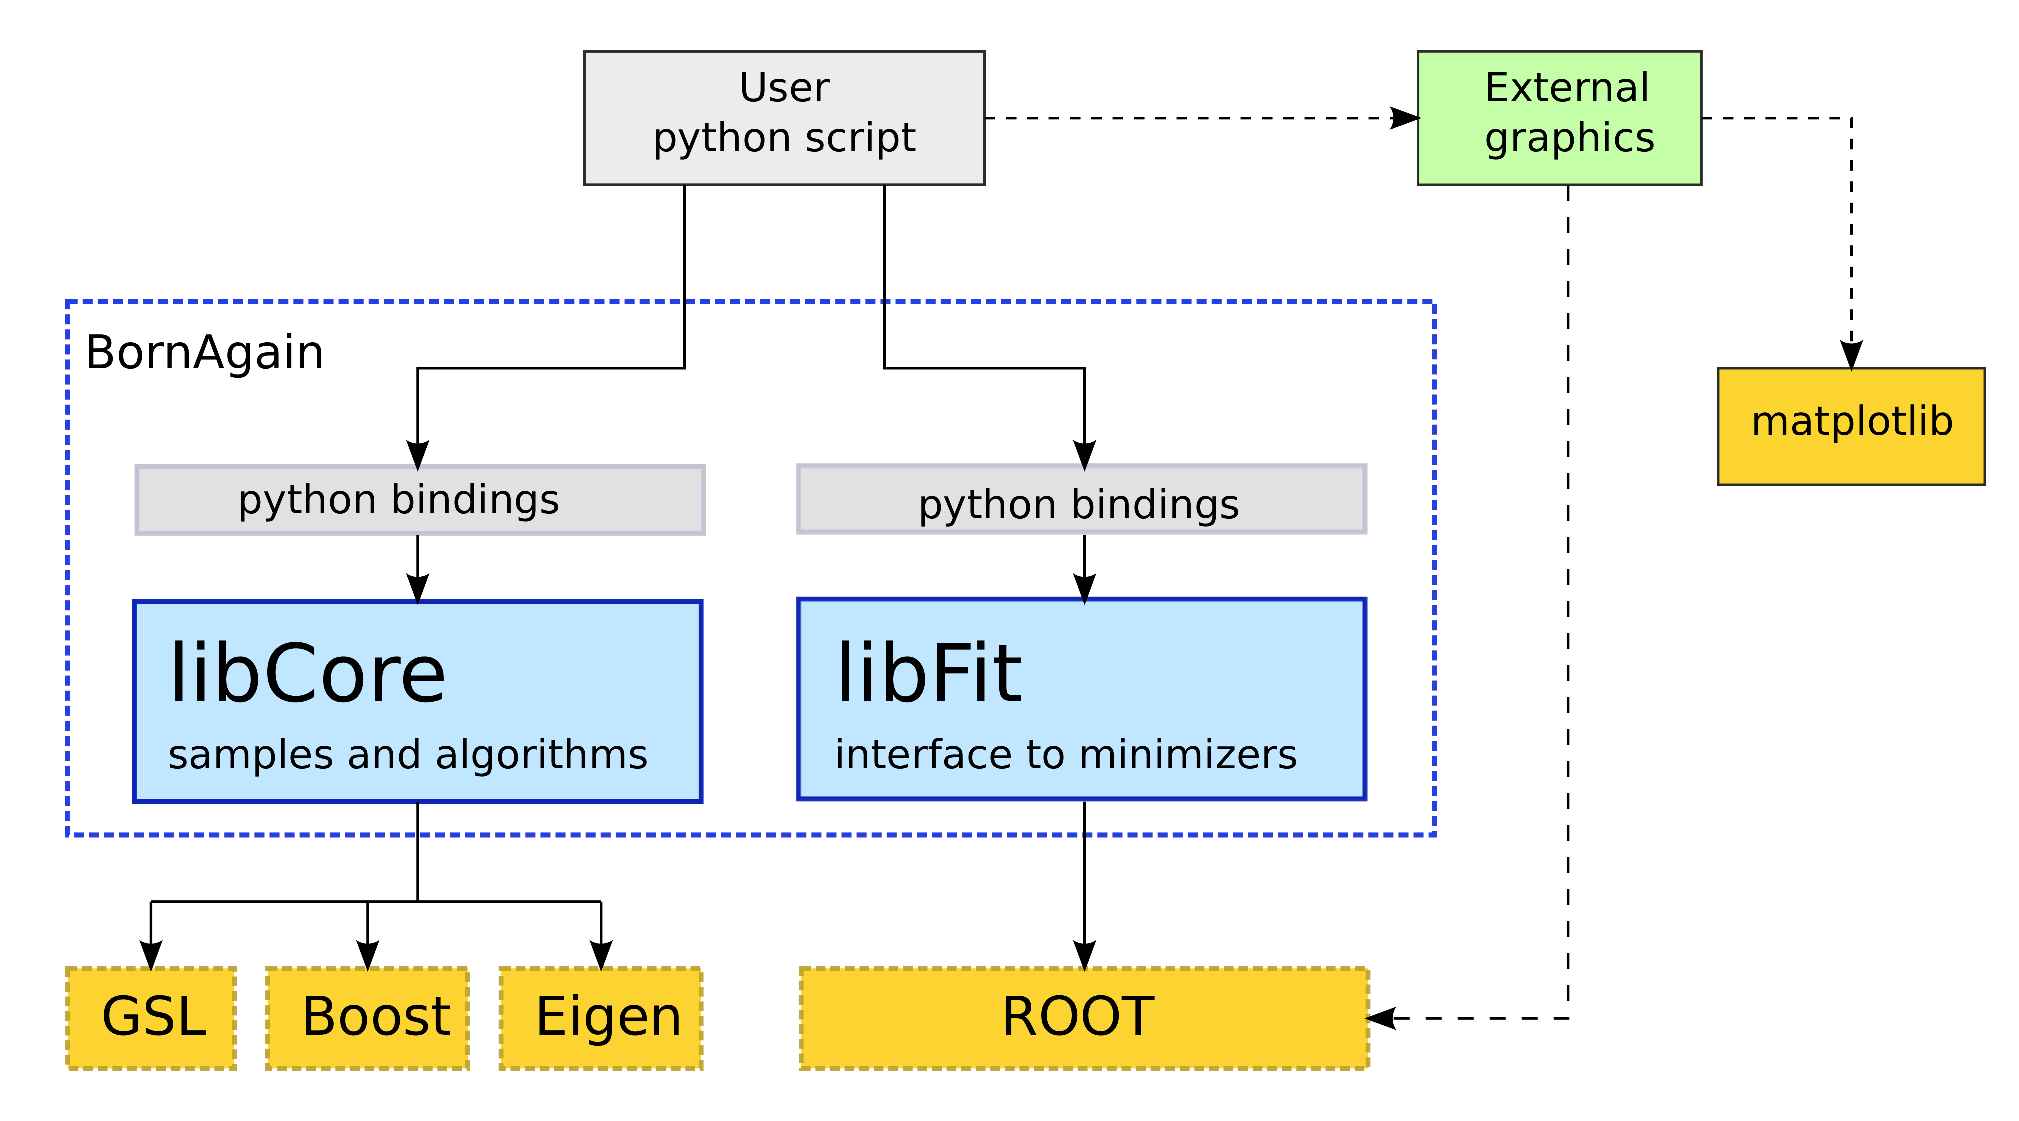
\includegraphics{Figures/basic_architecture.eps}}
\caption{
Structure of \BornAgain\ libraries.
}
\label{fig:two_ratios}
\end{figure}


The general structure of \BornAgain\ and the way user interacts with it are
shown in Fig.~\ref{fig:two_ratios}.
The framework kernel consists of two shared libraries, \Code{libCore} and
\Code{libFit}. Thanks to the python interface they can be imported to the python as external modules. The library \Code{libCore} contains a number of classes, grouped into several class categories necessary for the description of model and running the simulation.
The library  \Code{libFit} contains a number of minimization engines 
and interfaces to them, to let user to fit real data with the model defined.

\BornAgain\ depends from a few external well established open-source libraries: boost, GNU scientific library, Eigen and Fast Fourier Transformation libraries. They are required to be present on the system to run \BornAgain . Other libraries shown
on the plot (ROOT, matplotlib) are optional.

 



\section{Design overview}

% general considerations
% general capabilities and properties
% openess 
% global structure
% design and architecture

% Software process
% - configuration and release management
% - quality assurance and testing
% - user support process


% The BornAgain framework provides a number of classes, grouped into several class categories.


%%%%%%%%%%%%%%%%%%%%%%%%%%%%%%%%%%%%%%%%%%%%%%%%%%%%%%%%%%%%%%%%%%%%%%%%%%%%%%%%
%%
%%   BornAgain User Manual
%%
%%   homepage:   http://www.bornagainproject.org
%%
%%   copyright:  Forschungszentrum Jülich GmbH 2015
%%
%%   license:    Creative Commons CC-BY-SA
%%   
%%   authors:    Scientific Computing Group at MLZ Garching
%%               C. Durniak, M. Ganeva, G. Pospelov, W. Van Herck, J. Wuttke
%%
%%%%%%%%%%%%%%%%%%%%%%%%%%%%%%%%%%%%%%%%%%%%%%%%%%%%%%%%%%%%%%%%%%%%%%%%%%%%%%%%


\section{Data classes for simulations and fits}

This section will give an overview of the classes that are used to describe all the data needed to perform a single simulation. The prime elements of this data are formed by the sample, the experimental conditions (beam and detector parameters) and simulation parameters.

These classes constitute the main interface to the software's users, since they will mostly be interacting with the program by creating samples and running simulations with specific parameters. Since it is not the intent to explain internals of classes in this document, the text and figures will only mention the most important methods and fields of the classes discussed. Furthermore, getters and setters of private member fields will not be indicated, although these do belong to the public interface. For more detailed information about the project's classes, their methods and fields, the reader is referred to the source code documentation. REF?



\subsection{The Experiment object}
The \Code{Experiment} class holds all references to data objects that are needed to perform a simulation. These consist in a sample description, possibly implemented by a builder object, detector and beam parameters and finally, a simulation parameter class that defines the different approximations that can be used during a simulation. Besides getters and setters for these fields, the class also contains a \Code{runSimulation()} method that will generate an ISimulation object that will perform the actual computations. The class diagram for \Code{Experiment} is shown in \reffig{exp}.

\vspace{8mm}
\begin{figure}[H]
%the makebox macro ensures centering of the resulting figure
\makebox[\textwidth][c]{
\begin{tikzpicture}
\begin{umlpackage}{Simulation Data}
\umlclass{Experiment}{
  -- mp\_sample : ISample* \\
  -- mp\_sample\_builder : ISampleBuilder* \\
  -- m\_detector : Detector \\
  -- m\_beam : Beam \\
  -- m\_intensity\_map : OutputData<double> \\
  -- m\_sim\_params : SimulationParameters
}{
  \umlvirt{+ clone() : Experiment*} \\
  \umlvirt{+ runSimulation() : void} \\
  \umlvirt{+ normalize() : void}
}
\umlemptyclass[x=7, y=0]{ISample}
\umlemptyclass[x=7, y=-2]{Detector}
\umlemptyclass[x=7, y=-4]{Beam}
\umlemptyclass[x=7, y=-6]{SimulationParameters}
\umlemptyclass[y=-4]{GISASExperiment}
\umluniassoc[geometry=|-, anchor1=0]{Experiment}{ISample}
\umluniassoc[geometry=|-, anchor1=0]{Experiment}{Detector}
\umluniassoc[geometry=|-, anchor1=0]{Experiment}{Beam}
\umluniassoc[geometry=|-, anchor1=0]{Experiment}{SimulationParameters}
\umlinherit[geometry=--]{GISASExperiment}{Experiment}

\umlnote[y=-6.5, width=6cm]{GISASExperiment}{
  The ``runSimulation()'' method retrieves an ISimulation object
  from the topmost ISample object and calls its ``run()'' method 
  to perform the actual computations.
}
\end{umlpackage}
\end{tikzpicture}
} %end makebox
\caption{The Experiment class as a container for sample, beam, detector and simulation parameters.}
\label{fig:exp}
\end{figure}

\subsection{The ISample class hierarchy}

Samples are described by a hierarchical tree of objects which all adhere to the ISample interface. The composite pattern is used to achieve a common interface for all objects in the sample tree. The sample description is maximally decoupled from all computational classes, with the exception of the ``createDWBASimulation()'' method. This method will create a new object of type ``DWBASimulation'' that is capable of calculating the scattering contributions originating from the sample part in question. This coupling is not very tight however, since the ISample subclasses only need to know about which class to instantiate and return.

This interface and two of its subclasses are sketched in \reffig{isample}.

\vspace{8mm}

\begin{figure}[H]
\makebox[\textwidth][c]{
\begin{tikzpicture}
\begin{umlpackage}{Sample description} 
% Code from official documentation goes here...
\umlinterface{ISample}{
}{
  \umlvirt{+ clone() : ISample*} \\
  \umlvirt{+ createDWBASimulation() : DWBASimulation*}
}
\umlclass[y=-4]{MultiLayer}{
  -- m\_layers : std::vector<Layer *> \\
  -- m\_interfaces : std::vector<LayerInterface *>
}{
  + getNumberOfLayers() : size\_t \\
  + getNumberOfInterfaces() : size\_t \\
  + addLayer(const Layer \&layer) : void
}
\umlclass[x=8,y=-4]{Layer}{
  -- mp\_material : IMaterial* \\
  -- m\_thickness : double
}{
  + getThickness() : double \\
  + setThickness(double thickness) : void
}
\umlinherit[geometry=-|]{MultiLayer}{ISample}
\umlinherit[geometry=|-]{Layer}{ISample}
\umluniassoc[geometry=--, mult2=n]{MultiLayer}{Layer}
\end{umlpackage}
\end{tikzpicture}
}
\caption{The ISample interface}
\label{fig:isample}
\end{figure}



\subsection{The FitSuite class} \SecLabel{FitSuiteClass}

\subsection{The IMinimizer class} \SecLabel{IMinimizerClass}

\subsection{The MinimizerOptions class} \SecLabel{MinimizerOptionsClass}


\appendix
%\newpage{\pagestyle{empty}\cleardoublepage}


\chapter{Listings}

%%%%%%%%%%%%%%%%%%%%%%%%%%%%%%%%%%%%%%%%%%%%%%%%%%%%%%%%%%%%%%%%%%%%%%%%%%%%%%%%%%%%%%%%%%%%%%%%%%
%
%%%%%%%%%%%%%%%%%%%%%%%%%%%%%%%%%%%%%%%%%%%%%%%%%%%%%%%%%%%%%%%%%%%%%%%%%%%%%%%%%%%%%%%%%%%%%%%%%%
\section{Python simulation example} \label{PythonSimulationExampleScript}
The following script can be found at
\begin{lstlisting}[language=shell, style=commandline]
./Examples/python/simulation/ex001_CylindersAndPrisms/CylindersAndPrisms.py
\end{lstlisting}


\begin{lstlisting}[
language=python, 
style=eclipse, 
escapeinside={@}{@},
frame = leftline, 
rulecolor = \color{lightgrey},
breaklines = true
]
import numpy
import matplotlib
import pylab
from libBornAgainCore import *


def get_sample():
    """
    Build and return the sample representing cylinders and pyramids on top of
    substrate without interference.
    """
    # defining materials
    m_air = HomogeneousMaterial("Air", 0.0, 0.0)
    m_substrate = HomogeneousMaterial("Substrate", 6e-6, 2e-8)
    m_particle = HomogeneousMaterial("Particle", 6e-4, 2e-8)

    # collection of particles
    cylinder_ff = FormFactorCylinder(5*nanometer, 5*nanometer)
    cylinder = Particle(m_particle, cylinder_ff)
    prism_ff = FormFactorPrism3(10*nanometer, 5*nanometer)
    prism = Particle(m_particle, prism_ff)
    particle_layout = ParticleLayout()
    particle_layout.addParticle(cylinder, 0.0, 0.5)
    particle_layout.addParticle(prism, 0.0, 0.5)
    interference = InterferenceFunctionNone()
    particle_layout.addInterferenceFunction(interference)

    # air layer with particles and substrate form multi layer
    air_layer = Layer(m_air)
    air_layer.setLayout(particle_layout)
    substrate_layer = Layer(m_substrate, 0)
    multi_layer = MultiLayer()
    multi_layer.addLayer(air_layer)
    multi_layer.addLayer(substrate_layer)
    return multi_layer


def get_simulation():
    """
    Create and return GISAXS simulation with beam and detector defined
    """
    simulation = Simulation()
    simulation.setDetectorParameters(100, -1.0*degree, 1.0*degree, 100, 0.0*degree, 2.0*degree)
    simulation.setBeamParameters(1.0*angstrom, 0.2*degree, 0.0*degree)
    return simulation


def run_simulation():
    """
    Run simulation and plot results
    """
    sample = get_sample()
    simulation = get_simulation()
    simulation.setSample(sample)
    simulation.runSimulation()
    result = simulation.getIntensityData().getArray() + 1  # for log scale
    pylab.imshow(numpy.rot90(result, 1), norm=matplotlib.colors.LogNorm(), extent=[-1.0, 1.0, 0, 2.0])
    pylab.show()


if __name__ == '__main__':
    run_simulation()

\end{lstlisting}


%%%%%%%%%%%%%%%%%%%%%%%%%%%%%%%%%%%%%%%%%%%%%%%%%%%%%%%%%%%%%%%%%%%%%%%%%%%%%%%%%%%%%%%%%%%%%%%%%%
%
%%%%%%%%%%%%%%%%%%%%%%%%%%%%%%%%%%%%%%%%%%%%%%%%%%%%%%%%%%%%%%%%%%%%%%%%%%%%%%%%%%%%%%%%%%%%%%%%%%
\newpage
\section{Python fitting example} \label{PythonFittingExampleScript}

The following script can be found at
\begin{lstlisting}[language=shell, style=commandline]
./Examples/python/fitting/ex002_FitCylindersAndPrisms/FitCylindersAndPrisms.py
\end{lstlisting}

\begin{lstlisting}[
language=python, 
style=eclipse, 
frame = leftline, 
rulecolor = \color{lightgrey},
breaklines = true
]
from libBornAgainCore import *
from libBornAgainFit import *


def get_sample():
    """
    Build the sample representing cylinders and pyramids on top of substrate without interference.
    """
    # defining materials
    m_air = HomogeneousMaterial("Air", 0.0, 0.0)
    m_substrate = HomogeneousMaterial("Substrate", 6e-6, 2e-8)
    m_particle = HomogeneousMaterial("Particle", 6e-4, 2e-8)

    # collection of particles
    cylinder_ff = FormFactorCylinder(1.0*nanometer, 1.0*nanometer)
    cylinder = Particle(m_particle, cylinder_ff)
    prism_ff = FormFactorPrism3(2.0*nanometer, 1.0*nanometer)
    prism = Particle(m_particle, prism_ff)
    particle_layout = ParticleLayout()
    particle_layout.addParticle(cylinder, 0.0, 0.5)
    particle_layout.addParticle(prism, 0.0, 0.5)
    interference = InterferenceFunctionNone()
    particle_layout.addInterferenceFunction(interference)

    # air layer with particles and substrate form multi layer
    air_layer = Layer(m_air)
    air_layer.setLayout(particle_layout)
    substrate_layer = Layer(m_substrate, 0)
    multi_layer = MultiLayer()
    multi_layer.addLayer(air_layer)
    multi_layer.addLayer(substrate_layer)
    return multi_layer


def get_simulation():
    """
    Create GISAXS simulation with beam and detector defined
    """
    simulation = Simulation()
    simulation.setDetectorParameters(100, -1.0*degree, 1.0*degree, 100, 0.0*degree, 2.0*degree)
    simulation.setBeamParameters(1.0*angstrom, 0.2*degree, 0.0*degree)
    return simulation


def run_fitting():
    """
    run fitting
    """
    sample = get_sample()
    simulation = get_simulation()
    simulation.setSample(sample)

    real_data = IntensityDataIOFactory.readIntensityData('refdata_fitcylinderprisms.txt')
    
    fit_suite = FitSuite()
    fit_suite.addSimulationAndRealData(simulation, real_data)
    fit_suite.initPrint(10)

    # setting fitting parameters with starting values
    fit_suite.addFitParameter("*FormFactorCylinder/height", 4.*nanometer, 0.01*nanometer, AttLimits.lowerLimited(0.01))
    fit_suite.addFitParameter("*FormFactorCylinder/radius", 6.*nanometer, 0.01*nanometer, AttLimits.lowerLimited(0.01))
    fit_suite.addFitParameter("*FormFactorPrism3/height", 4.*nanometer, 0.01*nanometer, AttLimits.lowerLimited(0.01))
    fit_suite.addFitParameter("*FormFactorPrism3/length", 12.*nanometer, 0.02*nanometer, AttLimits.lowerLimited(0.01))

    # running fit
    fit_suite.runFit()
    
    print "Fitting completed."
    fit_suite.printResults()
    print "chi2:", fit_suite.getMinimizer().getMinValue()
    fitpars = fit_suite.getFitParameters()
    for i in range(0, fitpars.size()):
        print fitpars[i].getName(), fitpars[i].getValue(), fitpars[i].getError()

if __name__ == '__main__':
    run_fitting()
\end{lstlisting}


%%%%%%%%%%%%%%%%%%%%%%%%%%%%%%%%%%%%%%%%%%%%%%%%%%%%%%%%%%%%%%%%%%%%%%%%%%%%%%%%
%%
%%   BornAgain User Manual
%%
%%   homepage:   http://www.bornagainproject.org
%%
%%   copyright:  Forschungszentrum Jülich GmbH 2015
%%
%%   license:    Creative Commons CC-BY-SA
%%   
%%   authors:    Scientific Computing Group at MLZ Garching
%%               C. Durniak, M. Ganeva, G. Pospelov, W. Van Herck, J. Wuttke
%%
%%%%%%%%%%%%%%%%%%%%%%%%%%%%%%%%%%%%%%%%%%%%%%%%%%%%%%%%%%%%%%%%%%%%%%%%%%%%%%%%


%Appendix
\chapter{Implemented classes}

\begin{itemize}
\item Particle decoration
\item Layer
\item MultiLayer
\item Simulation
\end{itemize}

\chapter{Form factors}
% plots of particles + orientation of the axes
% plots of the form factors

\begin{itemize}
\item Parallelepiped (\texttt{FormFactorParallelepiped})

\begin{equation}
F(\mathbf{q},R, H) = 4H R^2\exp(i q_z H/2) \text{sinc}(q_xR)
\text{sinc}(q_yR)\text{sinc}(q_z H/2)
\end{equation}
%%%%%%%%%%%%%%%%%%%%%%%%%%%%%%%%%%%
\item Pyramid (\texttt{FormFactorPyramid})

\begin{align*}
        q_1 &=\frac{1}{2}\Big[\frac{q_x-q_y}{\tan(\alpha)} + q_z\Big],\quad       q_2 =\frac{1}{2}\Big[\frac{q_x-q_y}{\tan(\alpha)} - q_z\Big]\quad
        q_3 =\frac{1}{2}\Big[\frac{q_x+q_y}{\tan(\alpha)} + q_z\Big]\quad       q_4 =\frac{1}{2}\Big[\frac{q_x+q_y}{\tan(\alpha)} - q_z\Big]\\
        K_1 &= \text{sinc}(q_1 H)\exp(i q_1 H)  + i \text{sinc}(q_2 H) \exp(-i q_2 H)\\
        K_2 &= -i \text{sinc}(q_1 H) \exp(i q_1 H) +i
        \text{sinc}(q_2 H) \exp(-i q_2 H)\\
        K_3 &= \text{sinc}(q_3 H) \exp(i q_3 H)    +
        \text{sinc}(q_4 H) \exp(-i q_4 H)\\
        K_4 &= -i \text{sinc}(q_3 H) \exp(i q_3 H) + i \text{sinc}(q_4 H) \exp(-i q_4 H)\\     
  F(\mathbf{q},R, H, \alpha) &= \frac{H}{q_x q_y} \Big\{ K_1 \cos[ (q_x-q_y)R ] + K_2 \sin[ (q_x-q_y)R ] - K_3 \cos[ (q_x+q_y) R ] - K_4 \sin[ (q_x+q_y) R ]\Big\}
   \end{align*}
%%%%%%%%%%%%%%%%%%%%%%%%%%%%%%%%%%%%	
\item Cylinder (\texttt{FormFactorCylinder})

  \begin{equation}
 F(\mathbf{q},R, H)=   H  \text{sinc}(q_ z H/2) \exp(i q_ z H/2) 2\pi R^2 \frac{J_1(|q_{\parallel} R |)}{|q_{\parallel} R| }
 \end{equation}
 
%%%%%%%%%%%%%%%%%%%%%%%%%%%%%%%%%%%%
\item Prism3 (\texttt{FormFactorPrism3})

\begin{align*}
    F(\mathbf{q},R, H) &= 2 \sqrt{3}\frac{\exp(-i q_y
      R/\sqrt{3})}{q_x^2-3q_y^2} \Big[\exp(i \sqrt{3} q_y R )
    -\cos(q_x R)-i \sqrt{3} q_y R \text{sinc}(q_x R) \Big] \\
   &\times  H \text{sinc}(q_z H/2 ) \exp(i q_z H/2)
\end{align*}

%%%%%%%%%%%%%%%%%%%%%%%%%%%%%%%%%%%%
\item Sphere (\texttt{FormFactorSphere})

\begin{equation}    
F(\mathbf{q},R, H)= 2\pi \exp[i q_z (H-R)]\int_{R-H} ^{R} R_z^2 \frac{J_1(|q_{\parallel}
  R_z|) }{|q_{\parallel} R_z|}
        \exp(i q_z z) dz
\end{equation}

$R_z=\sqrt{R^2-z^2}$, $q_{\parallel}=\sqrt{q_x^2+q_y^2}$

%%%%%%%%%%%%%%%%%%%%%%%%%%%%%%%%%%%%
\item Full sphere (\texttt{FormFactorFullSphere})

\begin{equation}
F(\mathbf{q},R) = 4\pi R^3 \frac{\sin(q R) - q R \cos(q R)}{(qR)^3}
\end{equation}
%%%%%%%%%%%%%%%%%%%%%%%%%%%%%%%%%%%%
\item Box (\texttt{FormFactorBox})

\begin{equation}
F(\mathbf{q},R,W,H)= 4H R W\exp(i q_z H/2) \text{sinc}(q_x R) \text{sinc}(q_y W) \text{sinc}(q_z H/2)
\end{equation}
    
where $\text{sinc}(x)=\sin(x)/x$ is the cardinal sine, $J_1(x)$ is the
Bessel function of first order.
	
\end{itemize}

\chapter{Interference functions}

\begin{itemize}
\item	No interference 
\item	decoupling approximation 	
\item 	local mono disperse approximation 
\item 	size spacing approximation 
\end{itemize}


\chapter{Pair correlation functions}
\begin{itemize}
\item The Debye hard core 
\item The gaussian
\item The Lennard-Jones  	
\item The gate pair correlation 	
\item The Debye hard core with power-law decrease  	
\item The Zhu pair correlation function 	
\item The Venables pair correlation function 	
\item The bidimensional hard core pair function.
\end{itemize}

%\bibliographystyle{switch}
\bibliographystyle{unsrt}
\bibliography{jw7}

\end{document}
